% !TEX program=pdflatex
% LaTeX rebuttal letter example. 
% 
% Copyright 2019 Friedemann Zenke, fzenke.net
%
% Based on examples by Dirk Eddelbuettel, Fran and others from 
% https://tex.stackexchange.com/questions/2317/latex-style-or-macro-for-detailed-response-to-referee-report
% 
% Licensed under cc by-sa 3.0 with attribution required.

\documentclass[12pt]{article}
\usepackage[utf8]{inputenc}
\usepackage{lipsum} % to generate some filler text
\usepackage{fullpage}
\usepackage{times}
\usepackage{amsmath, amsthm, amsfonts}
\usepackage{booktabs}
\usepackage{makecell}
\usepackage{multirow}
\usepackage{lscape}
\usepackage{xcolor}
\usepackage{float}
\usepackage{subfig}
\usepackage{graphicx}
\usepackage{framed}
\usepackage[colorlinks=true]{hyperref}
% Vector
\newcommand{\MyVec}[1]{\boldsymbol{#1}}
% Matrix
\newcommand{\MyMat}[1]{\boldsymbol{#1}}
% Vectors with hat
\newcommand{\hvec}[1]{\hat{\boldsymbol{h}}_{#1}}
% Model parameters
\newcommand{\Param}[1]{\textcolor{blue}{#1}}

\usepackage{blindtext}
\usepackage[most]{tcolorbox} 
\definecolor{block-gray}{gray}{0.95}


\newtcolorbox{zitat}[2][]{%
    colback=block-gray,
    grow to right by=-10mm,
    grow to left by=-10mm, 
    boxrule=0pt,
    boxsep=0pt,
    breakable,
    enhanced jigsaw,
    borderline west={4pt}{0pt}{gray},
    title={#2\par},
    colbacktitle={block-gray},
    coltitle={black},
    fonttitle={\large\bfseries},
    attach title to upper={},
    #1,
}

\newenvironment{myquote}[1]%
{\vspace{0.5em}\begin{zitat}{#1}}
{\end{zitat}\vspace{0.5em}}


% import Eq and Section references from the main manuscript where needed
% \usepackage{xr}
% \externaldocument{manuscript}

% package needed for optional arguments
\usepackage{xifthen}
% define counters for reviewers and their points
\newcounter{reviewer}
\setcounter{reviewer}{0}
\newcounter{point}[reviewer]
\setcounter{point}{0}

% This refines the format of how the reviewer/point reference will appear.
\renewcommand{\thepoint}{P\,\thereviewer.\arabic{point}} 

% command declarations for reviewer points and our responses
\newcommand{\reviewersection}{\stepcounter{reviewer} \bigskip \hrule
                  \section*{Reviewer \thereviewer}}

\newenvironment{point}
   {\refstepcounter{point} \bigskip \noindent {\textbf{Reviewer~Point~\thepoint} } ---\ \begin{sf}}
   {\end{sf} \par}

\newcommand{\shortpoint}[1]{\refstepcounter{point}  \bigskip \noindent 
	{\textbf{Reviewer~Point~\thepoint} } ---\begin{sf} ~#1 \end{sf}\par}

\newenvironment{reply}
   {\medskip \noindent \textbf{Reply}:\  }
   {\medskip}

\newcommand{\shortreply}[2][]{\medskip \noindent \textbf{Reply}:\  #2
	\ifthenelse{\equal{#1}{}}{}{ \hfill \footnotesize (#1)}%
	\medskip}

\begin{document}

\section*{Response to the Reviewers}
% General intro text goes here
We thank the reviewers for their critical assessment and insightful comments of our work.
%
We have made extensive modifications to our manuscript.
%
In the following we address their concerns point by point.
%
We also prepare an \emph{annotated version} for our revised manuscript.
%
In the annotated version, changes corresponding to each point are all highlighted by red squares.

\subsection*{Summary of Changes}

%%%% TODO %%%

% Let's start point-by-point with Reviewer 1
\reviewersection

% R1Q0
\begin{point}
    The authors conduct an empirical analysis of performance bottlenecks in graph neural network training. The authors identify the edge-related calculation is the performance bottleneck. Experimental of several GNN variants, such as GCN, GGNNNN, GAT and GaAN on six real-world graph datasets verify the importance of the findings. The experimental analysis is sufficient. However, there are some tiny issues in this paper.
\end{point}

\begin{reply}
    Thank you for your positive comments on our manuscript.
    %
    We have carefully revised the manuscript according to your comments. 
    %
    Based on the suggestions, we have made an extensive modification on the revised manuscript.
    %
    Please see the detailed responses below.
    %
    The changes corresponding to each issue were highlighted by red squares in the annotated version of our manuscript.

\end{reply}

% R1Q1
\begin{point}
	There are lots of symbols in this paper. Some symbols are reused and confusing, such as s denotes sub-layers or edge features.
\end{point}

% Our reply
\begin{reply}
    We apologize for the confusing use of symbols and thank you for pointing the problem out.
    %
    To clarify the symbol usage, we have checked the manuscript and unified the usage of symbol.
    %
    We avoid the problem of reusing symbols, so that each symbol only represents one meaning after the revision.
    %
    We summarize the frequently-used symbols in Table 1 in the revised manuscript.
    %
    We quote the table below:
    \begin{table}[H]
        \footnotesize
        \centering
        \begin{tabular}{p{3em}lp{35em}}
            \toprule
            Category & Symbol & Meaning \\
            \midrule
            \multirow[c]{4}{3em}{Graph Structure}& $\mathcal{G}=(\mathcal{V}, \mathcal{E})$ & The simple undirected input graph with the vertex set $\mathcal{V}$ and the edge set $\mathcal{E}$. \\
            & $v_x$ & The $x$-th vertex of the input graph. \\
            & $e_{y,x}$ & The edge pointing from $v_y$ to $v_x$ of the input graph. \\
            & $\mathcal{N}(v_x)$ & The adjacency set of $v_x$ in the input graph. \\ 
            & $\bar{d}$ & The average degree of the input graph. \\ \midrule
            \multirow[c]{6}{3em}{GNN Definition}& $L$ & The number of GNN layers. \\
            & $K$ & The number of heads in a GNN layer. \\
            & $\phi^l$ & The messaging function of the GNN layer $l$. \\
            & $\Sigma^l$ & The aggregation function of the GNN layer $l$. \\
            & $\gamma^l$ & The vertex updating function of the GNN layer $l$. \\ 
            & $\phi^{l,i}$ / $\Sigma^{l,i}$ / $\gamma^{l,i}$ & The messaging/aggregation/updating function of the $i$-th sub-layer of the GNN layer  $l$.\\
            & $\textcolor{blue}{\boldsymbol{W}^l, \boldsymbol{W}^{(k)}/\boldsymbol{b}, \boldsymbol{a}}$ & The matrices/vectors represented by the blue characters are the weight matrices/vectors that need to be learned in the GNN. \\  \midrule
            \multirow[c]{8}{3em}{Vector}& $\boldsymbol{v}_x$ & The feature vector of the vertex $v_x$. \\
            & $\boldsymbol{e}_{y,x}$ & The feature vector of the edge $e_{y,x}$.  \\
            & $\boldsymbol{h}_x^{l}$ &  The {input} hidden vector of the graph neuron corresponding to $v_x$ in the GNN layer $l$. \\
            & $\boldsymbol{h}_x^{l+1}$ &  The {output} hidden vector of the graph neuron corresponding to $v_x$ in the GNN layer $l$.\\
            & $\boldsymbol{m}_{y,x}^l$ & The message vector of the edge $e_{y,x}$ outputted by $\phi^l$ of the GNN layer $l$. \\
            & $\boldsymbol{s}_{x}^l$ & The aggregated vector of the vertex $v_x$ outputted by $\Sigma^l$ of the GNN layer $l$. \\
            & $\boldsymbol{h}_{x}^{l,i}$ / $\boldsymbol{m}_{y,x}^{l,i}$ / $\boldsymbol{s}_{x}^{l,i}$ & The hidden/message/aggregated vector of the vertex $v_x$ outputted by $\gamma^{l,i}$/$\phi^{l,i}$/$\Sigma^{l,i}$ of the $i$-th sub-layer of the GNN layer $l$. \\
            & $d^l_{in}$, $d^l_{out}$ &  The dimension of the input/output hidden vectors of the GNN layer $l$. \\
            & $dim(\MyVec{x})$ & The dimension of a vector $\MyVec{x}$. \\
            \bottomrule
        \end{tabular}
\end{table}

    
    In the revised manuscript, we use $e_{y,x}$ to represent an edge and use $\boldsymbol{e}_{y,x}$ to represent its input feature vector.
    %
    The input feature vectors of all edges are same for all GNN layers.
    %
    We use $\boldsymbol{s}$ to represent aggregated vectors outputted by the aggregation function $\Sigma$ in graph neurons.
    %
    For every vertex $v_x$, we use $\boldsymbol{s}^l_x$ to denote its aggregated vector in the GNN layer $l$.
    %
    If the GNN layer $l$ has sub-layers, $\boldsymbol{s}^{l,i}_x$ represents its aggregated vector in the $i$-th sub-layer.
    
    To clarify the concept of \emph{sub-layers} in a GNN layer, we have added more description on it in the revised manuscript.
    %
    We first introduce the concept of sub-layer in Section 2.2 ``Graph Neuron and Message-passing Model'' as:
    %
    \begin{myquote}{Section 2.2}
        Some complex GNNs like GAT [6] and GaAN [7] use more than one message passing phase in each GNN layer.
        %
        We regard every message passing phase in a GNN layer as a \emph{sub-layer}.
        %
        We will give out more details on sub-layers when we introduce GAT.
    \end{myquote}
    %
    We then use GAT as an example to elaborate on the concept of sub-layers in Section 2.3 ``Representative GNNs'' as:
    %
    \begin{myquote}{Section 2.3}
        \newcommand{\GATCalcWeight}{\exp(LeakyReLU(\Param{\MyVec{a}}^T[\hvec{y}[k] \parallel \hvec{x}[k]]))}
        Each GAT layer consists of a vertex pre-processing phase and two sub-layers (i.e., message-passing phases).
        
        The vertex pre-processing phase calculates the attention vector $\hat{\boldsymbol{h}}^{l}_{x}$ for every vertex $v_x$ by $\hvec{x} = \parallel_{k=1}^K \Param{\MyMat{W}^l_{(k)}}\MyVec{h}^l_x$. We denote the attention sub-vector generated by the $k$-th head as $\hvec{x}[k]=\Param{\MyMat{W}^l_{(k)}}\MyVec{h}^l_x$.
        
        The first sub-layer of GAT (defined in Equation~\ref{eq:GAT-sub-layer-1}) uses the attention vectors to emit the attention weight vector $\boldsymbol{m}^{l,0}_{y,x}$ for every edge $e_{y,x}$ and aggregates the attention weight vectors for every vertex $v_x$ to get the weight sum vector $\MyVec{h}^{l,0}_x$.
        %
        \begin{equation}
            \footnotesize
            \label{eq:GAT-sub-layer-1}
            \begin{aligned}
                \MyVec{m}^{l,0}_{y,x} & = \phi^{l,0}(\MyVec{h}^l_y, \MyVec{h}^l_x, \MyVec{e}_{y,x}, \hvec{y}, \hvec{x}) = \parallel_{k=1}^{K}\GATCalcWeight, \\
                \MyVec{s}^{l,0}_{x} &= {\Sigma}_{v_y \in \mathcal{N}(v_x)}{\MyVec{m}^{l,0}_{y,x}}, \\
                \MyVec{h}^{l,0}_{x} &= \gamma^{l,0}(\MyVec{h}^l_x, \MyVec{s}^{l,0}_{x})  = \MyVec{s}^{l,0}_{x}.
            \end{aligned}
        \end{equation}
        %
        The second sub-layer of GAT (defined in Equation~\ref{eq:GAT-sub-layer-2}) uses the weight sum vectors to normalize the attention weights for every edge and aggregates the attention vectors $\boldsymbol{\hat{h}}^l_y$ with the normalized weights.
        %
        The aggregated attention vectors $\MyVec{s}^{l,1}_x$ are transformed by an activation function $\delta$ and are outputted as the hidden vectors of the current layer $\MyVec{h}^{l+1}_x$.
        %
        \begin{equation}
            \footnotesize
            \label{eq:GAT-sub-layer-2}
            \begin{aligned}
                \MyVec{m}^{l,1}_{y,x} &= \phi^{l,1}(\MyVec{h}^{l,0}_y, \MyVec{h}^{l,0}_x, \MyVec{e}_{y,x}, \hvec{y}, \hvec{x}) = \parallel_{k=1}^{K}\frac{\GATCalcWeight}{\MyVec{h}^{l,0}_x[k]}\hvec{y}[k], \\
                \MyVec{s}^{l,1}_x &= {\Sigma}_{v_y \in \mathcal{N}(v_x)} \MyVec{m}^{l,1}_{y,x}, \\
                \MyVec{h}^{l+1}_x = \MyVec{h}^{l,1}_x &= \gamma^{l,1}(\MyVec{h}^{l,0}, \MyVec{s}^{l,1}_x) = \delta(\MyVec{s}^{l,1}_x).
            \end{aligned}
        \end{equation}
    \end{myquote}
\end{reply}

% R1Q2
\begin{point}
    Some typical applications of GNNs should be included, such as video object segmentation [ref1], human-object interaction [ref2] and human-parsing [ref3].[1] Zero-shot video object segmentation via attentive graph neural networks,iccv 2019 [2] Learning human-object interactions by graph parsing neural networks, eccv 2018. [3] Hierarchical human parsing with typed part-relation reasoning, cvpr 2020.
\end{point}

\begin{reply}
	Thank you for pointing out our shortcomings. Computer vision is indeed another important application area of graph neural networks. We have added the mentioned references in the INTRODUCTION section in the revised manuscript. We quote the related sentence below:
    \begin{myquote}{Section 1}
         The powerful expression ability makes GNNs achieve good accuracy in not only graph analytical tasks [8, 9, 10] (like node classification and link prediction) but also computer vision tasks (like human-object interaction [11], human parsing [12], and video object segmentation [13]).
    \end{myquote}
\end{reply}

% R1Q3
\begin{point}
There are some grammar errors and typos:
\\
  - `Take the demo GNN in Figure 1(a) as  the example.'
\\
 - `to calculate the  output hidden vector $h^{l+1}$ of the current layer l, i.e., $h^{l+1}$ = $\gamma^l(h^l,s^l)$ The end-to-end training requires…'
\\
 - `Implementing it with the specially optimized basic operators on the GPU is a potential optimization'
\\
 - The sentences in the experimental section should be unified.
\end{point}

\begin{reply}

    Thank you for pointing them out.
    %
    We feel really sorry for our carelessness.
    %
    We have proofread our revised manuscript carefully to eliminate grammar errors and typos.
    %
    We have also unified the tenses of the sentences in Section 3 ``Evaluation Design'' and Section 4 ``Evaluation Results and Analysis''.
    %
    We use the past tense to describe experimental methods, results and what they indicate.
    %
    We only use the present tense in the sentences that Figure/Table X are the subjects of the sentences.

\end{reply}

% R1Q4
\begin{point}
    Figures 6 and 7 should be adjusted. The figures and fonts are too small.
\end{point}

\begin{reply}
    
    Thank you for pointing the problem out.
    %
    Besides Figure 6 and Figure 7, we have adjusted all the figures in the revised manuscript to make sure that font sizes in figures are no less than the font size of figure captions.
    %
    To make the figures more easy to read, we also splitted Figure 6 and Figure 7 into five figures (Figure 6 to 10) in the revised manuscript to enlarge the subfigures.
    
\end{reply}

% R1Q5
\begin{point}
    In my view, computation efficiency is to describe the testing or validation process. Except for reporting and analyzing the training times, it is meaningful to discuss the inference time. This is also an important point of view for deep learning researchers to be concerned about.
\end{point}

\begin{reply}
    Thank you for the insightful comment and suggestion.
    %
    The efficiency of inference (including inference time and memory usage) is indeed important for deep learning researchers and engineers.
    %
    In the revised manuscript, we have added a new subsection (Section 2.5 ``Inference with GNNs'') in the revised manuscript to briefly review how to perform inference with GNNs.
    %
    To discuss the efficiency of GNN inference on GPUs, we have added corresponding analysis on GNN inference in every subsection of Section 4 ``Evaluation Results and Analysis''.
    %
    Below, we introduce our main findings subsection by subsection.
   
    \paragraph{Section 4.1 ''Effects of Hyper-parameters on Performance''}

    In Section 4.1 ``Effects of Hyper-parameters on Performance'', we have additionally measured how the time and the peak memory usage changed as we increased the values of the hyper-parameters during \emph{inference}.
    
    
    For all GNNs, we found that the effects of hyper-parameters on the \emph{inference time} were the same as the training time.
    %
    Taking GGNN as an example, Figure~\ref{fig:compare_effect_of_hyperparameter_on_time} in the response (Figure X and Figure X in the revised manuscript) compares the effects of the hidden vector dimension $dim(\MyVec{h}^1_x)$ on training/inference time.
    %
    As $dim(\MyVec{h}^1_x)$ increased, the vertex/edge calculation time of training time and inference time both grew linearly when the values of hyper-parameters were large enough.
    %
    We observed similar phenomena with the other GNNs.
    %
    The results indicated that the time complexity analysis of GNNs were applicable to both training and inference.
        
    \begin{figure}[H]
            \centering
             \subfloat[Training]{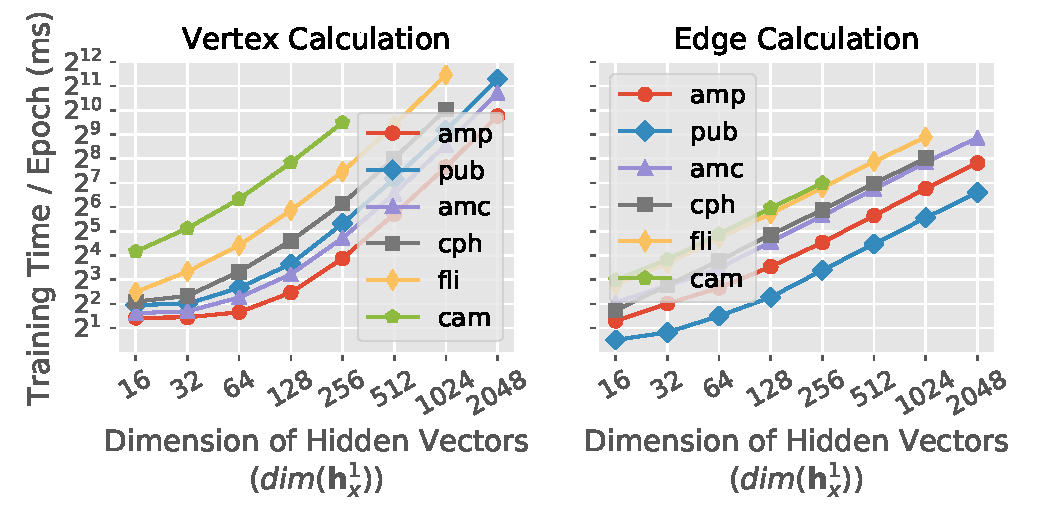
\includegraphics[width=0.7\textwidth]{../figs/experiments/exp_hyperparameter_on_vertex_edge_phase_time_ggnn.pdf}}\\
            \subfloat[Inference]{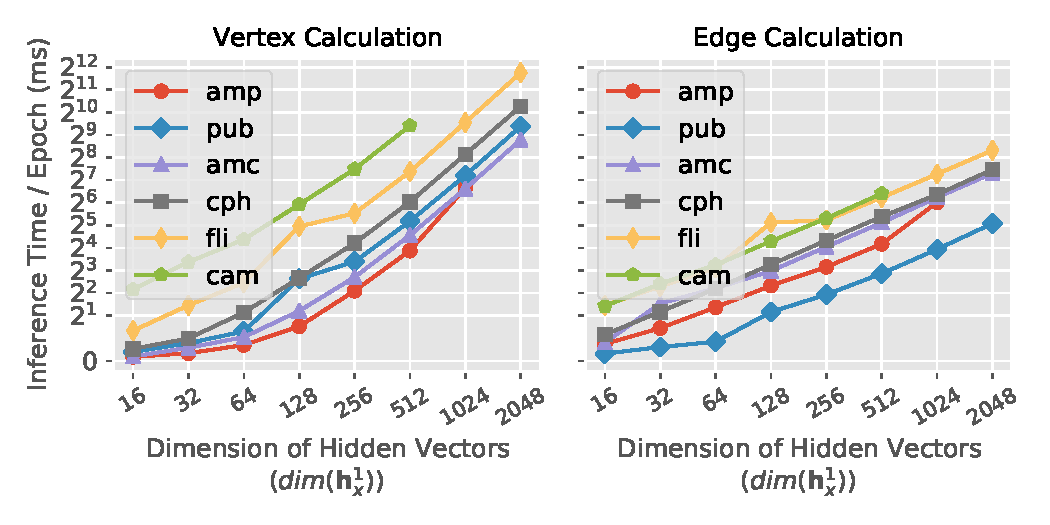
\includegraphics[width=0.7\textwidth]{../figs/experiments/exp_hyperparameter_on_inference_vertex_edge_phase_time_ggnn.pdf}}
            \caption{Effects of hyper-parameters on the vertex/edge calculation time of GGNN.}
            \label{fig:compare_effect_of_hyperparameter_on_time}
    \end{figure}
        
    For all GNNs, we found that the effects of hyper-parameters on inference memory usage were also same as training.
    %
    Taking GAT as an example, Figure~\ref{fig:compare_effect_of_hyperparameter_on_memory_usage} in the response (Figure X and Figure X in the revised manuscript) compares the peak memory usage during training and inference under different values of hyper-parameters.
        %
    The trends of the curves in Figure~\ref{fig:compare_effect_of_hyperparameter_on_memory_usage_training} and Figure~\ref{fig:compare_effect_of_hyperparameter_on_memory_usage_inference} were highly similar.
        %
    The memory usage of training and inference \emph{both} grew linearly as the dimension of each head and the number of heads increased.
        %
    We observed similar phenomena with the other GNNs.
        %
    \begin{figure}[H]
            \centering
            \subfloat[Training\label{fig:compare_effect_of_hyperparameter_on_memory_usage_training}]{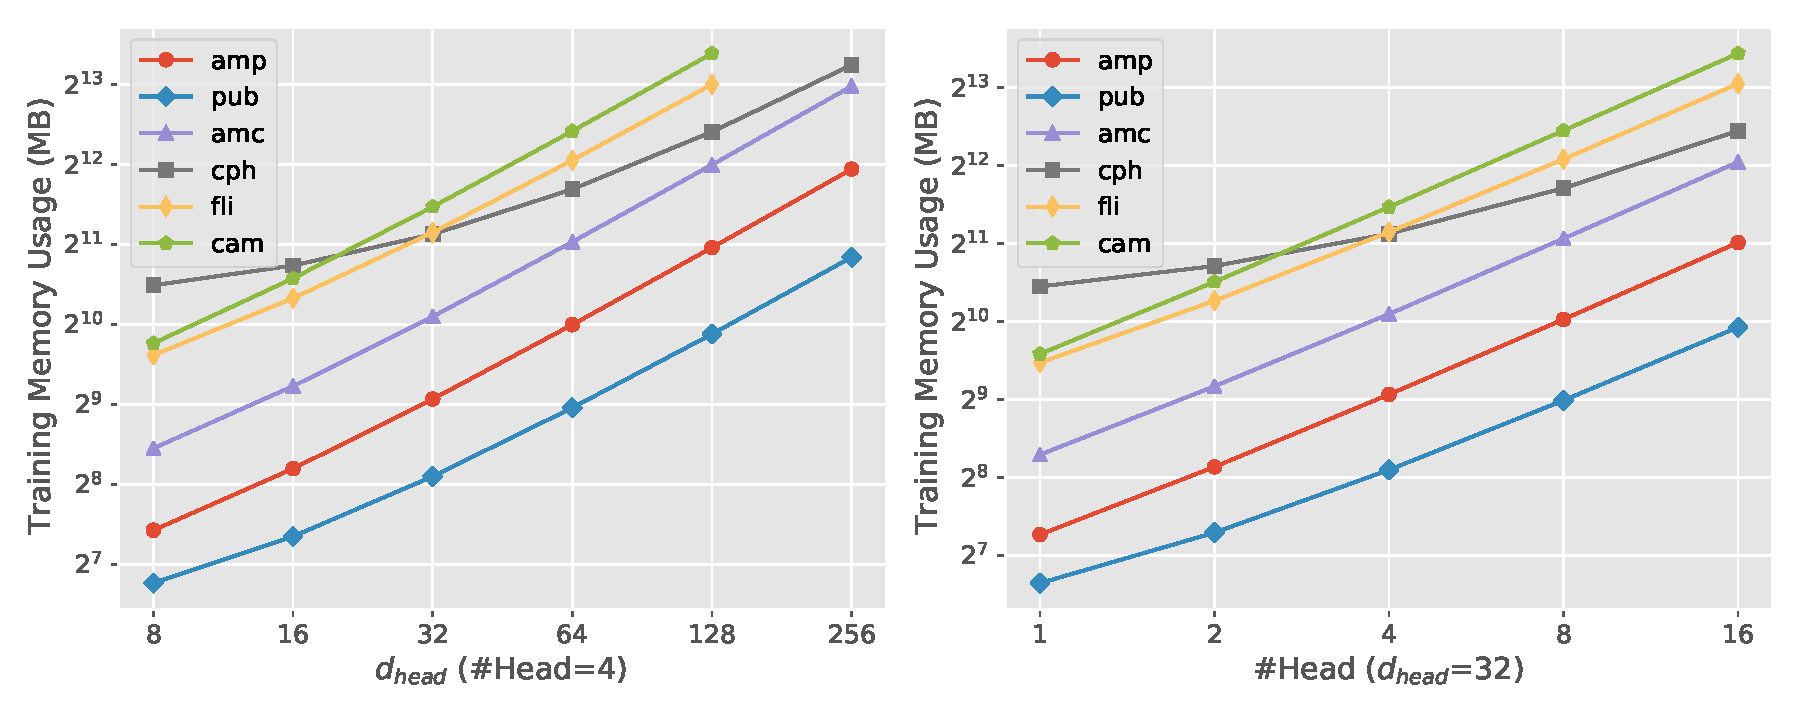
\includegraphics[width=0.6\textwidth]{../figs/experiments/exp_hyperparameter_on_memory_usage_gat.pdf}}\\
            \subfloat[Inference\label{fig:compare_effect_of_hyperparameter_on_memory_usage_inference}]{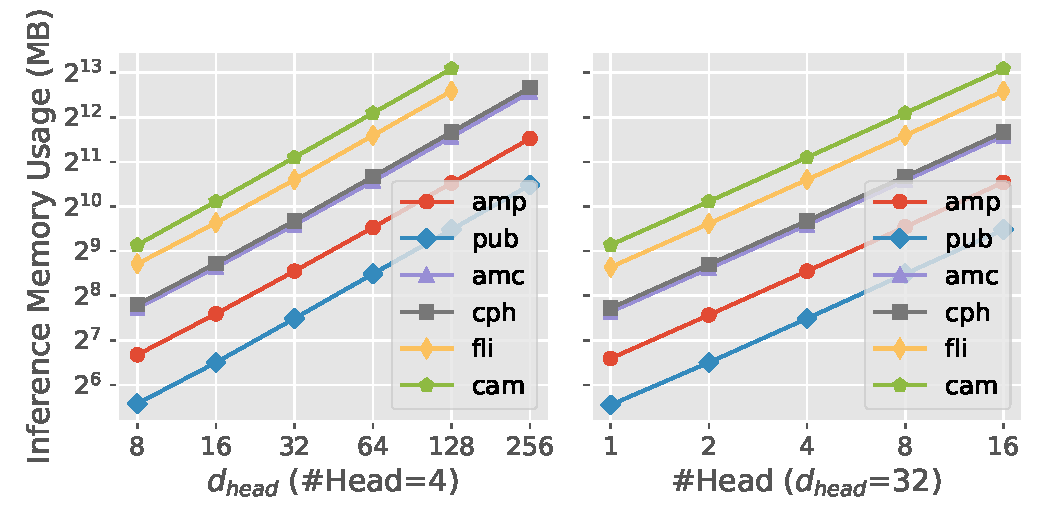
\includegraphics[width=0.6\textwidth]{../figs/experiments/exp_hyperparameter_on_inference_memory_usage_gat.pdf}}
            \caption{Effects of hyper-parameters on peak memory usage of GAT.}
            \label{fig:compare_effect_of_hyperparameter_on_memory_usage}
    \end{figure}
        
    \paragraph{Section 4.2 ``Time Breakdown Analysis''}    
    In Section 4.2 ``Time Breakdown Analysis'', we have additionally conducted the time breakdown analysis for GNN inference, in order to find out its performance bottlenecks.

    We found that the performance characteristics of GNN inference were highly similar to GNN training on the \emph{layer} level and the \emph{step} level.
    %
    In this reply, we used GCN as an example.
    %
    We made similar observations about the other GNNs.
    %
    Figure~\ref{fig:compare_layer_level_time_breakdown} in the response compares the time breakdowns of GCN on the layer level of training and inference.
    %
    The time breakdowns on the layer level were very similar between inference and training.
    %
    Figure~\ref{fig:compare_effect_of_degree} in the response compares the effects of the average degree on the proportion of edge/vertex calculation time during training and inference.
    %
    The curves in the two sub-figures of Figure~\ref{fig:compare_effect_of_degree} show very similar trends.
    %
    The results indicated that the edge calculation dominated both the training and inference time.
    %
    Figure~\ref{fig:compare_time_breakdown_of_edge_calculation} in the response further compares the time breakdowns on the step level of the edge calculation stage of GCN.
    %
    The proportion of each step was very similar in training and inference.
    %
    Therefore, \emph{the performance bottlenecks of training and inference were same on the layer level and step level}.
    
    \begin{figure}[H]
            \subfloat[Training]{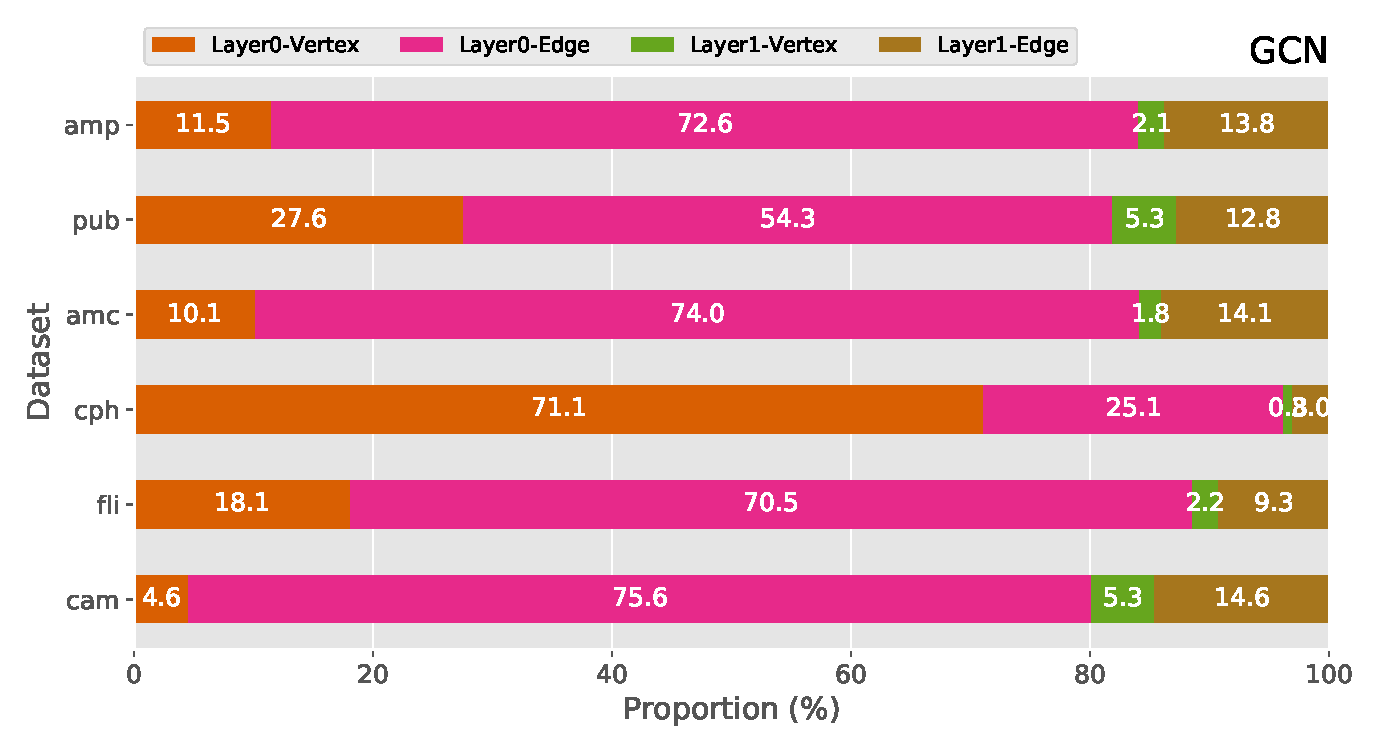
\includegraphics[width=0.5\columnwidth]{../figs/experiments/exp_layer_time_proportion_gcn.pdf}}
            \subfloat[Inference]{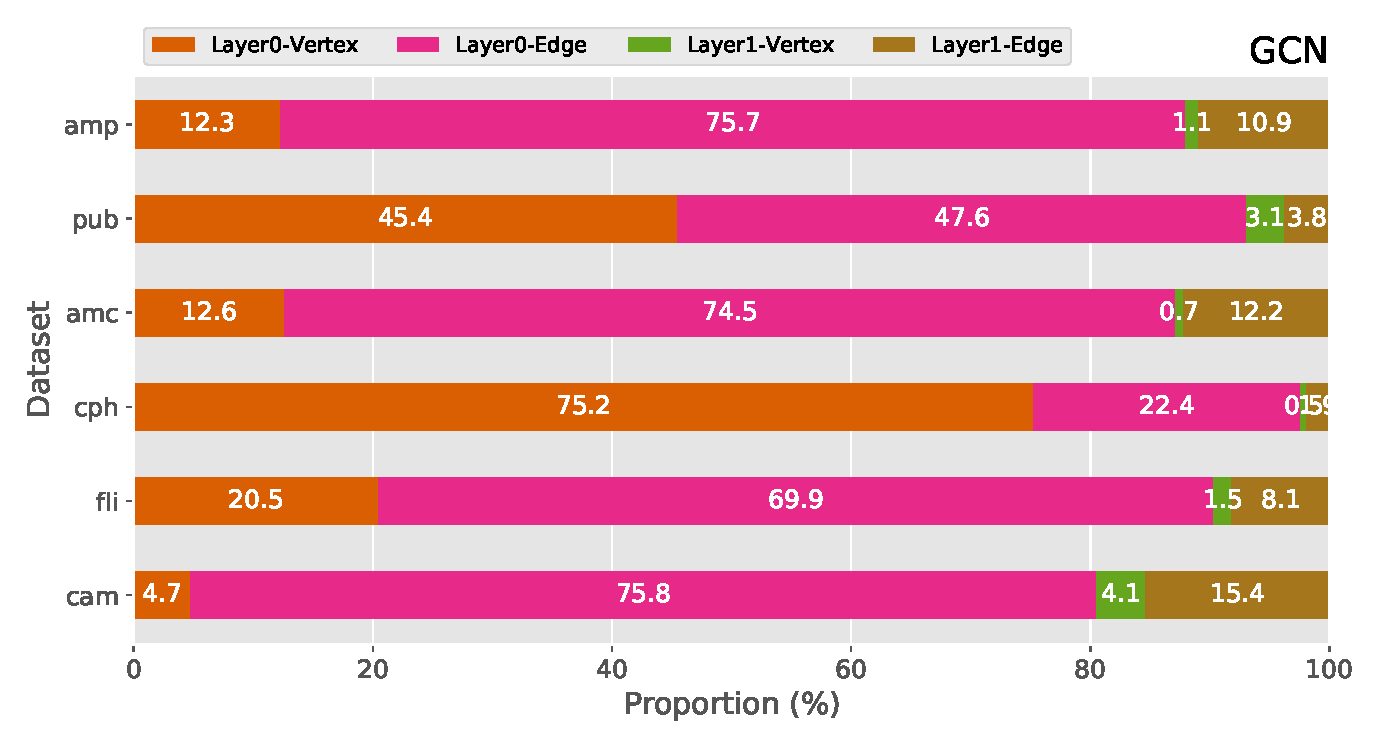
\includegraphics[width=0.5\columnwidth]{../figs/experiments/exp_inference_full_layer_time_proportion_gcn.pdf}}
            \caption{Time breakdowns on the layer level of GCN.}
            \label{fig:compare_layer_level_time_breakdown}
    \end{figure}
    %
    \begin{figure}[H]
                \subfloat[Training\label{fig:compare_effect_of_degree_training}]{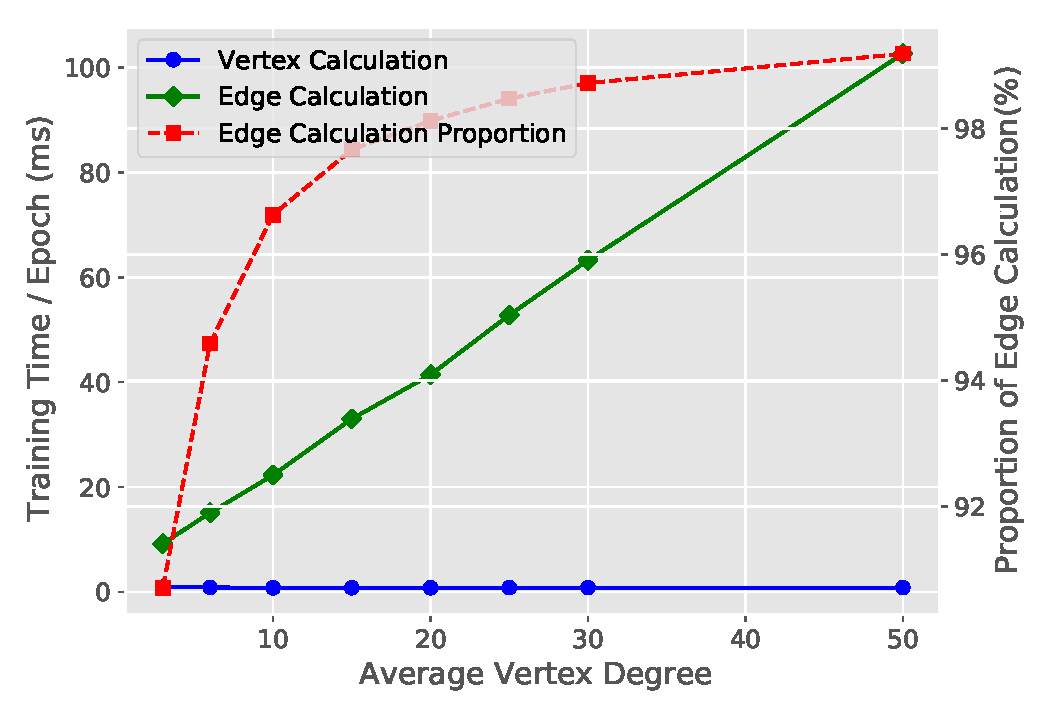
\includegraphics[width=0.5\columnwidth]{../figs/experiments/exp_avg_degree_on_vertex_edge_cal_time_gcn.pdf}}
                \subfloat[Inference\label{fig:compare_effect_of_degree_inference}]{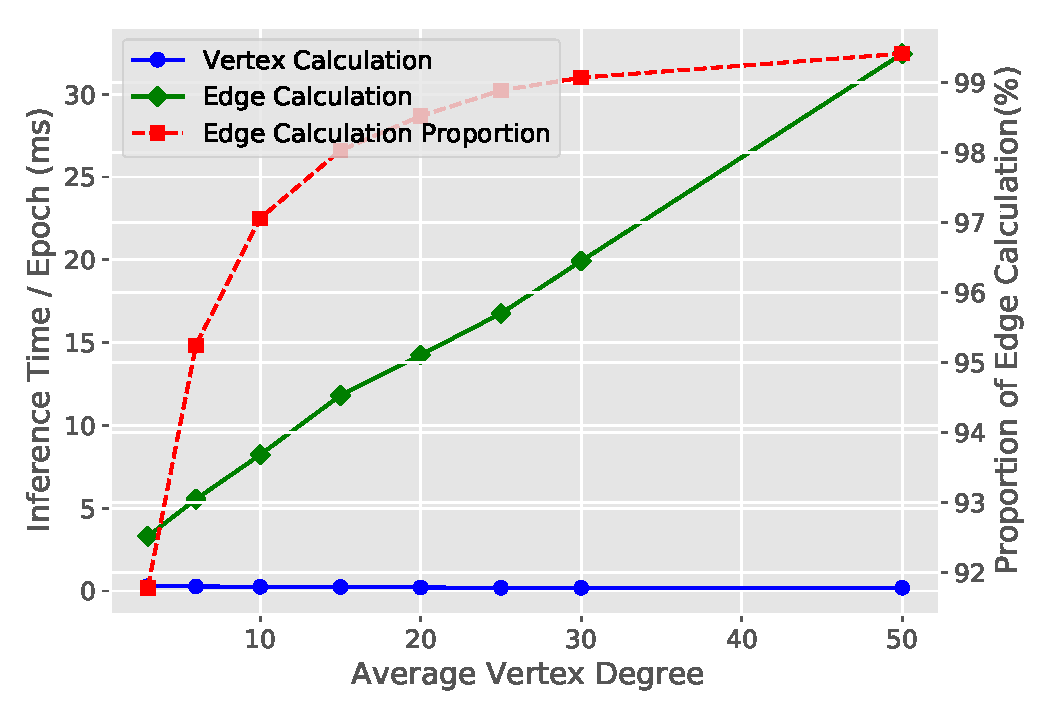
\includegraphics[width=0.5\columnwidth]{../figs/experiments/exp_inference_full_avg_degree_on_vertex_edge_cal_time_gcn.pdf}}
                \caption{Effects of the average degree on the proportion of the edge/vertex calculation time of GCN. Graphs were generated by fixing the number of vertices as 50,000.}
                \label{fig:compare_effect_of_degree}
    \end{figure}
    %
    \begin{figure}[H]
                \subfloat[Training]{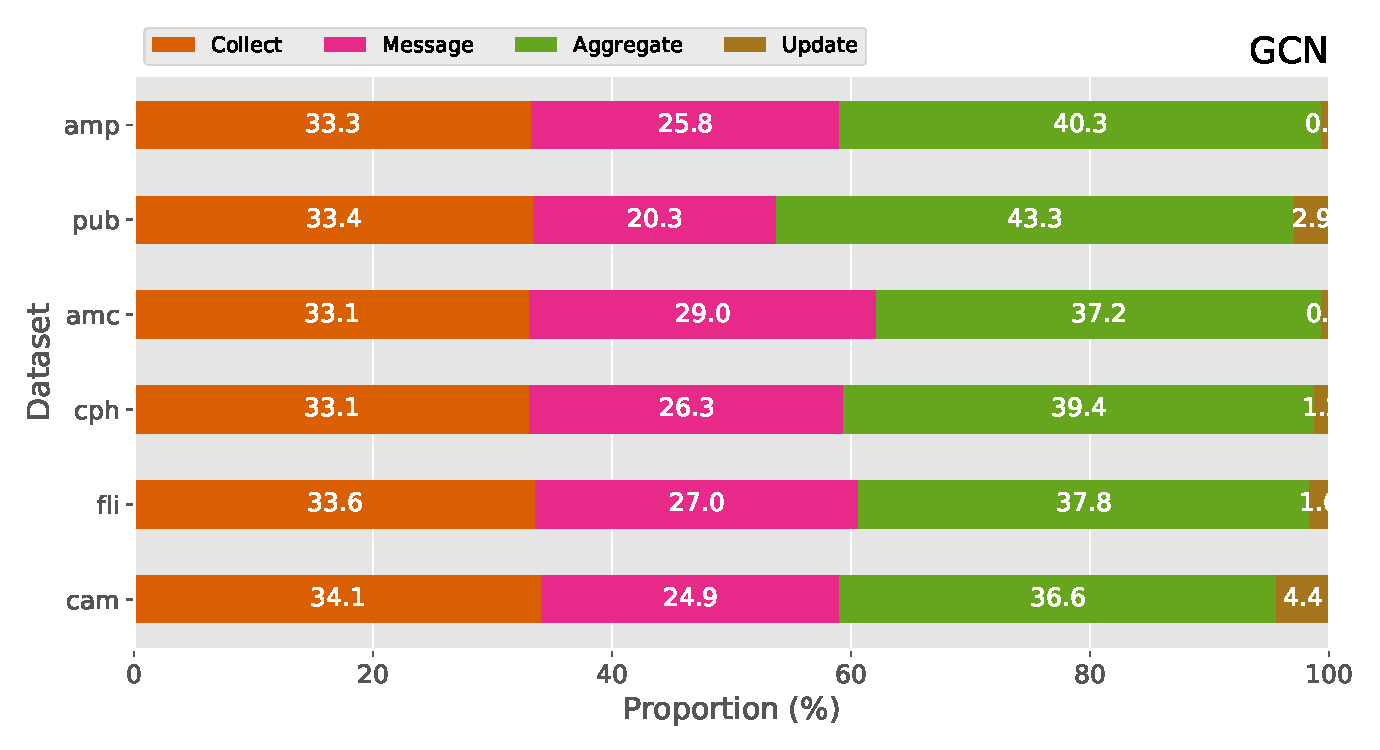
\includegraphics[width=0.5\columnwidth]{../figs/experiments/exp_edge_calc_decomposition_gcn.pdf}}
                \subfloat[Inference]{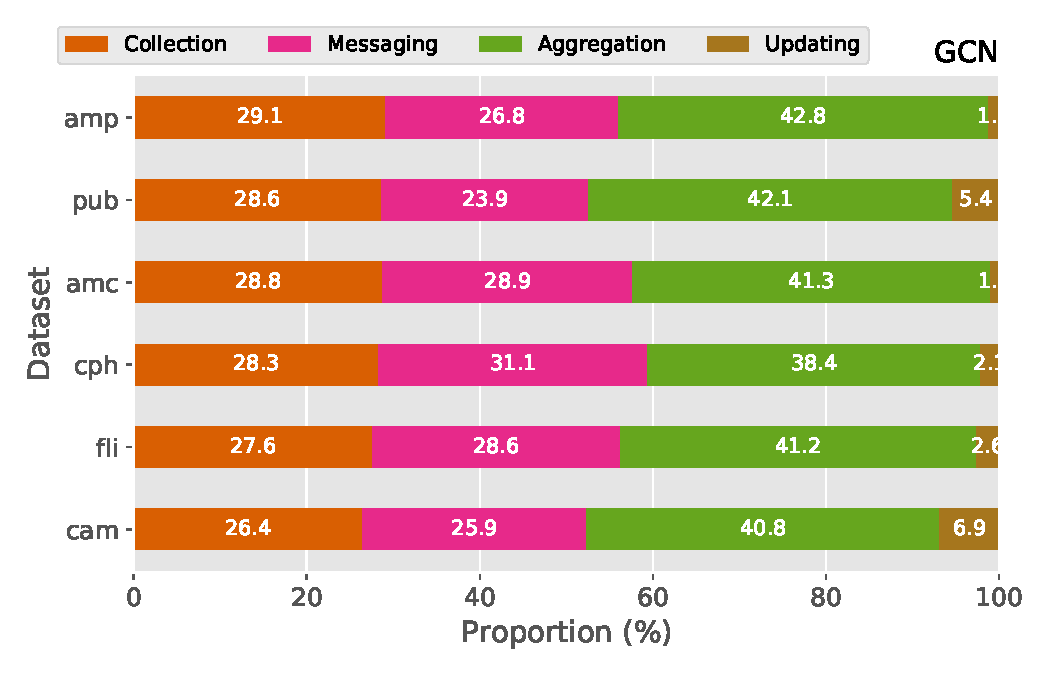
\includegraphics[width=0.5\columnwidth]{../figs/experiments/exp_inference_full_edge_calc_decomposition_gcn.pdf}}
                \caption{Time breakdowns on the step level of the edge calculation stage of GCN.}
                \label{fig:compare_time_breakdown_of_edge_calculation}
    \end{figure}
    
    The main differences between training and inference were reflected in two aspects: the wall-clock time and the top time-consuming basic operators.
    
    Figure~\ref{fig:compare_wall_clock_time_of_training_and_inference} in the response (Figure X in the revised manuscript) compares the wall-clock training/inference time on the \texttt{amp}, \texttt{amc}, and \texttt{fli} datasets.
    %
    The results on the other datasets were similar.
    %
    Since the inference only conducted the forward propagation from the input layer to the prediction layer, the time of inference was very close to the time of the forward phase in training.
    %
    The inference time was only 34\% (GCN), 32\% (GGNN), 25\% (GAT), and 32\% (GaAN) of the training time for the four GNNs, averaged over datasets.
    
    \begin{figure}[H]
        \centering
        \subfloat[\texttt{amc}]{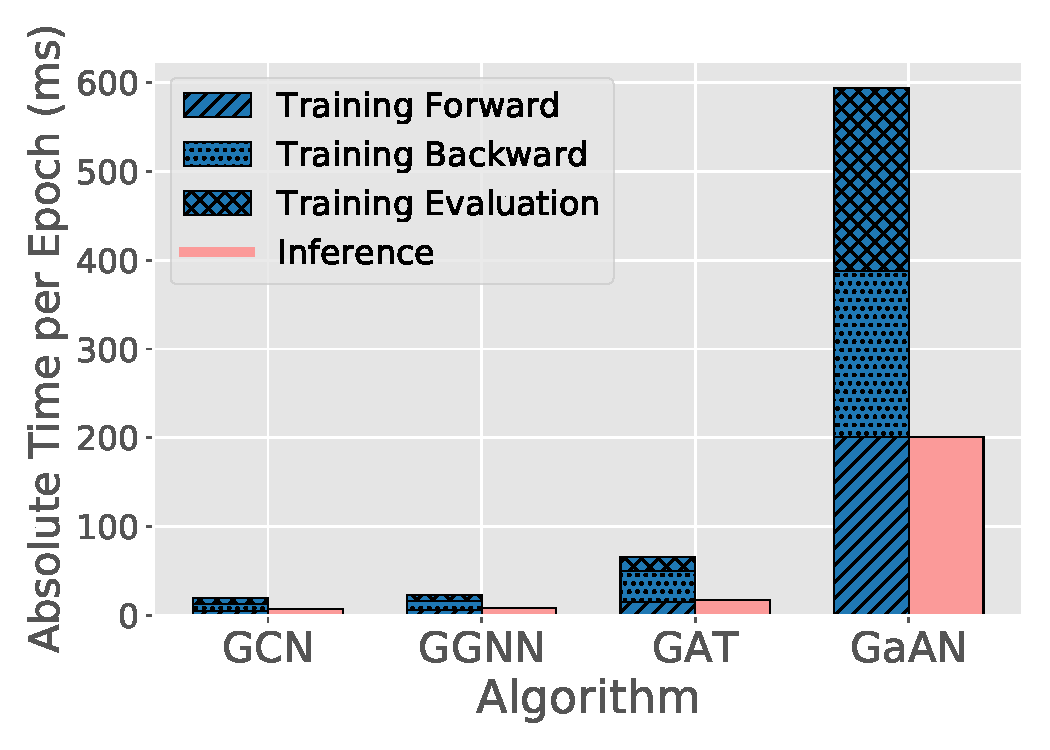
\includegraphics[width=0.3\columnwidth]{../figs/experiments/exp_time_comparison_between_training_inference_amazon-computers.pdf}}
        \subfloat[\texttt{amp}]{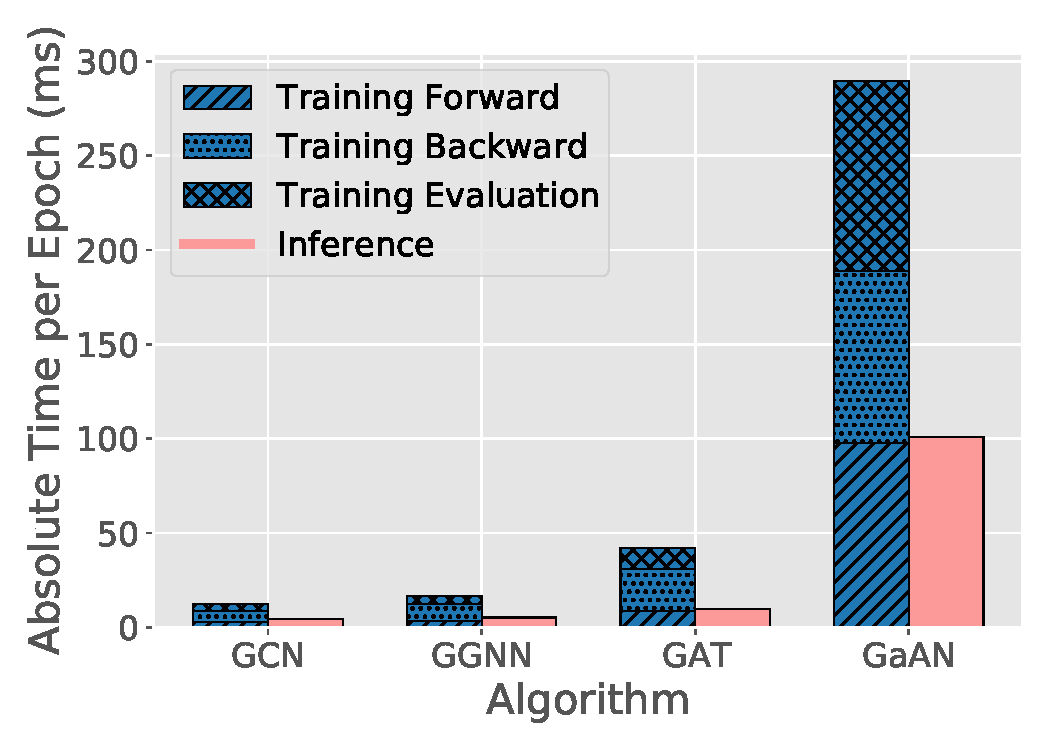
\includegraphics[width=0.3\columnwidth]{../figs/experiments/exp_time_comparison_between_training_inference_amazon-photo.pdf}}
        \subfloat[\texttt{fli}]{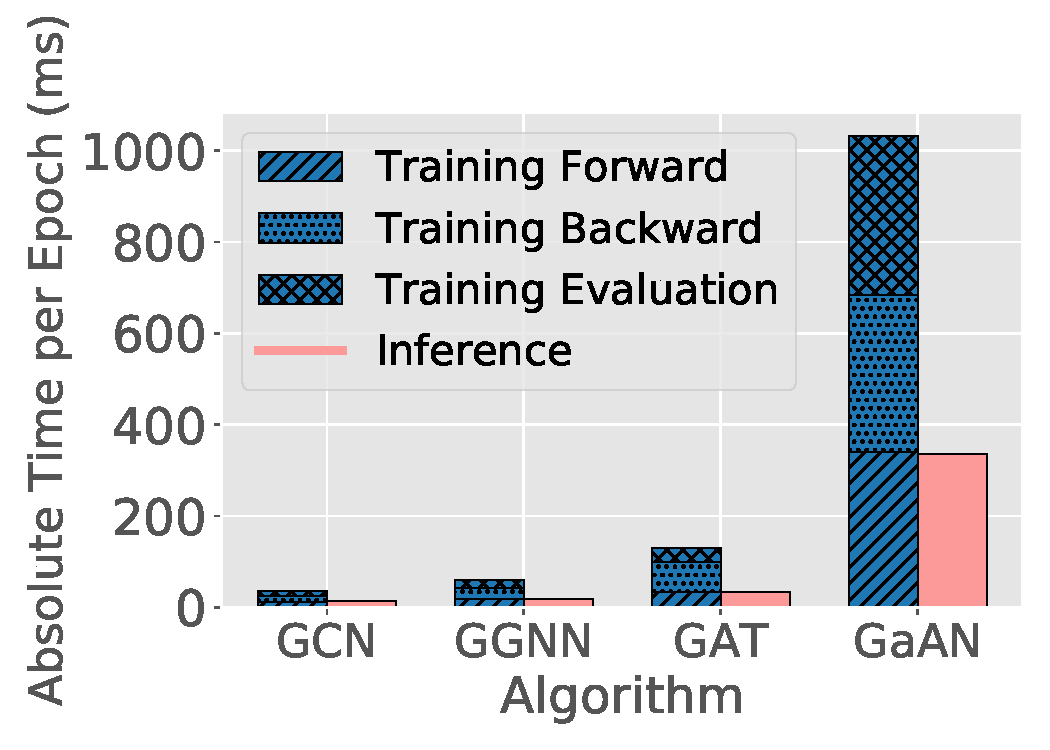
\includegraphics[width=0.3\columnwidth]{../figs/experiments/exp_time_comparison_between_training_inference_flickr.pdf}}
        \caption{Wall-clock training/inference time on different datasets.}
        \label{fig:compare_wall_clock_time_of_training_and_inference}
    \end{figure}
    
    The top time-consuming basic operators of training and inference showed a certain degree of difference.
    %
    In All GNNs, some of the top time-consuming operators during training were replaced by new operators in inference.
    %
    Figure~\ref{fig:compare_top_time_consuming_basic_operators} in the response compares the top 5 time-consuming basic operators in training and inference.
    %
    For GCN, the \texttt{index} operator that was used in the prediction layer became the new top 5 time-consuming operator, replacing the \texttt{gather} operator used in the backward phase in training.
    %
    The basic operators related to the edge calculation (\texttt{scatter\_add}, \texttt{index\_select}, and \texttt{mul}) still consumed the majority of the inference time.
    %
    For GGNN, \texttt{index} operator in the prediction layer also became one of the top 5 time-consuming basic operators.
    %
    Due to the high time complexity of the vertex updating function $\gamma$ in GGNN, the basic operators related to the vertex calculation stage (\texttt{mm} and \texttt{thnn\_fused\_gru\_cell}) still consumed near half of the inference time.
    %
    For GAT, the \texttt{input\_put\_impl} operator (used in the backward phase) in Figure~\ref{fig:compare_top_time_consuming_basic_operators}e was replaced by the \texttt{scatter\_add} operator in Figure~\ref{fig:compare_top_time_consuming_basic_operators}f.
    %
    The \texttt{scatter\_add} operator was still related to the edge calculation step.
    %
    For GaAN, the \texttt{mm} operator of GaAN was replaced by the \texttt{cat} operator used in the vertex updating function.
    
    Comparing the top basic operator distribution, GNN training and inference had common performance bottlenecks on the operator level.
    %
    The matrix multiplication \texttt{mm} and the element-wise multiplication \texttt{mul} operators were the common time-consuming operators, making GNN training and inference \emph{both suitable for GPUs}.
    %
    The basic operators related to the collection and aggregation steps in the edge calculation consumed consumed non-trivial time in both training and inference.
    
    \begin{figure}[H]
        \centering
        \subfloat[GCN, Training]{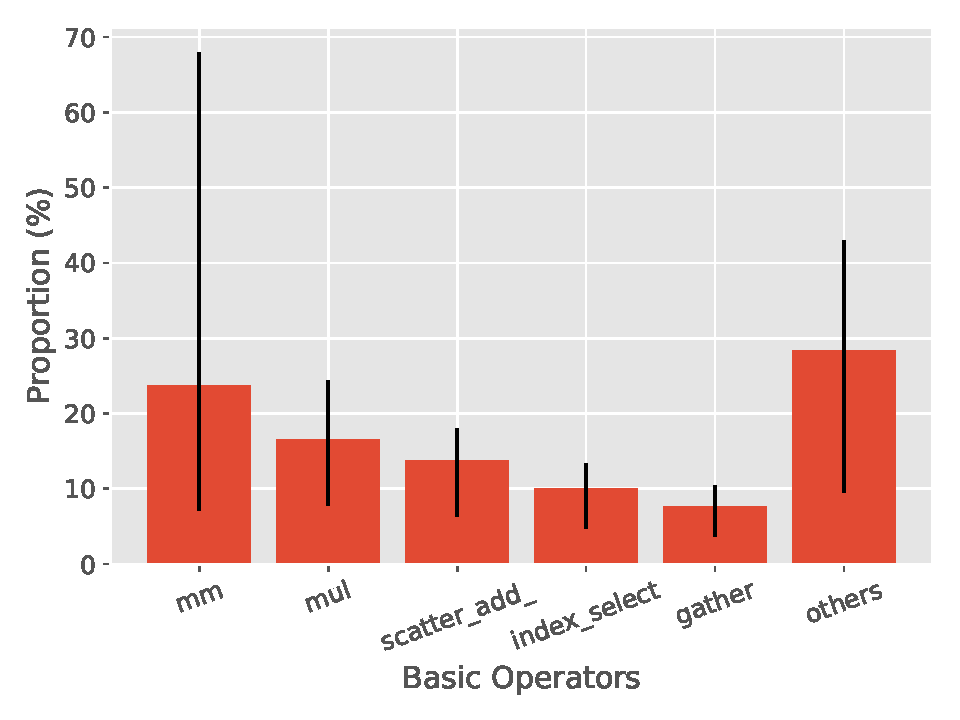
\includegraphics[width=0.35\columnwidth]{../figs/experiments/exp_top_basic_ops_gcn.pdf}}
         \subfloat[GCN, Inference]{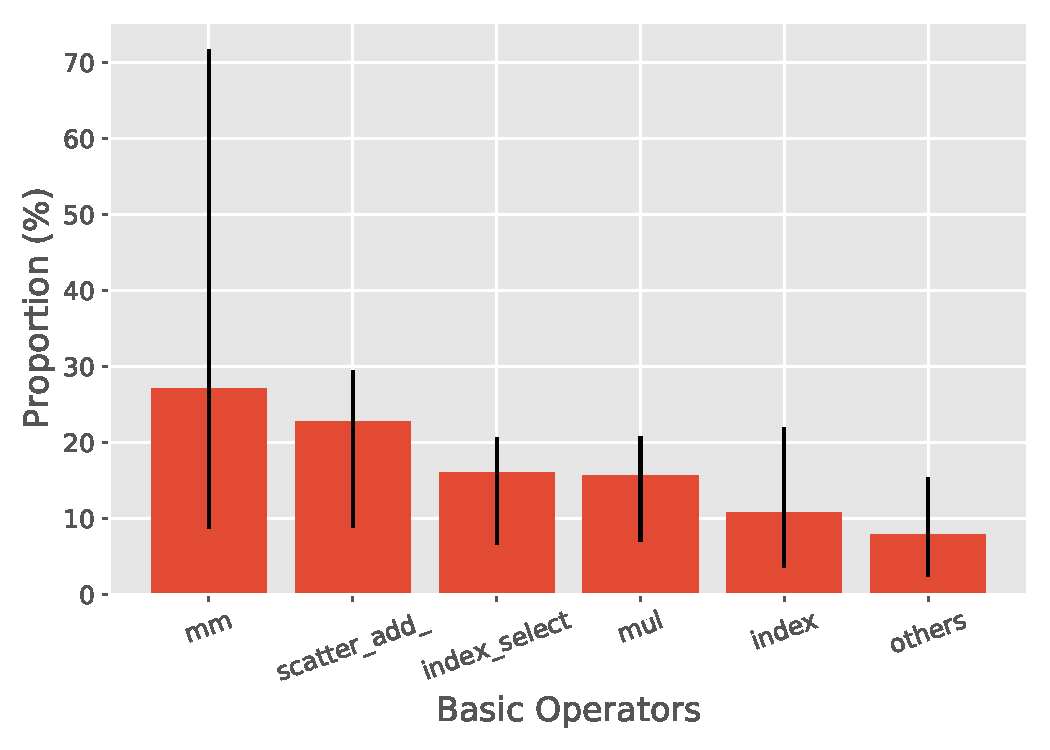
\includegraphics[width=0.35\columnwidth]{../figs/experiments/exp_inference_full_top_basic_ops_gcn.pdf}}\\
        \subfloat[GGNN, Training]{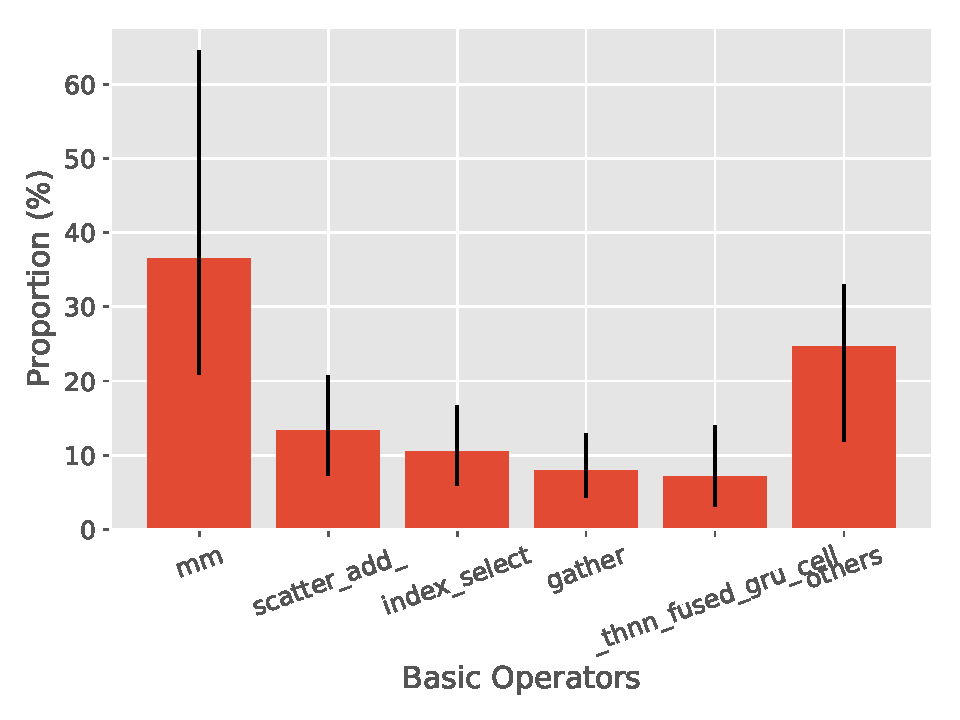
\includegraphics[width=0.35\columnwidth]{../figs/experiments/exp_top_basic_ops_ggnn.pdf}}
         \subfloat[GGNN, Inference]{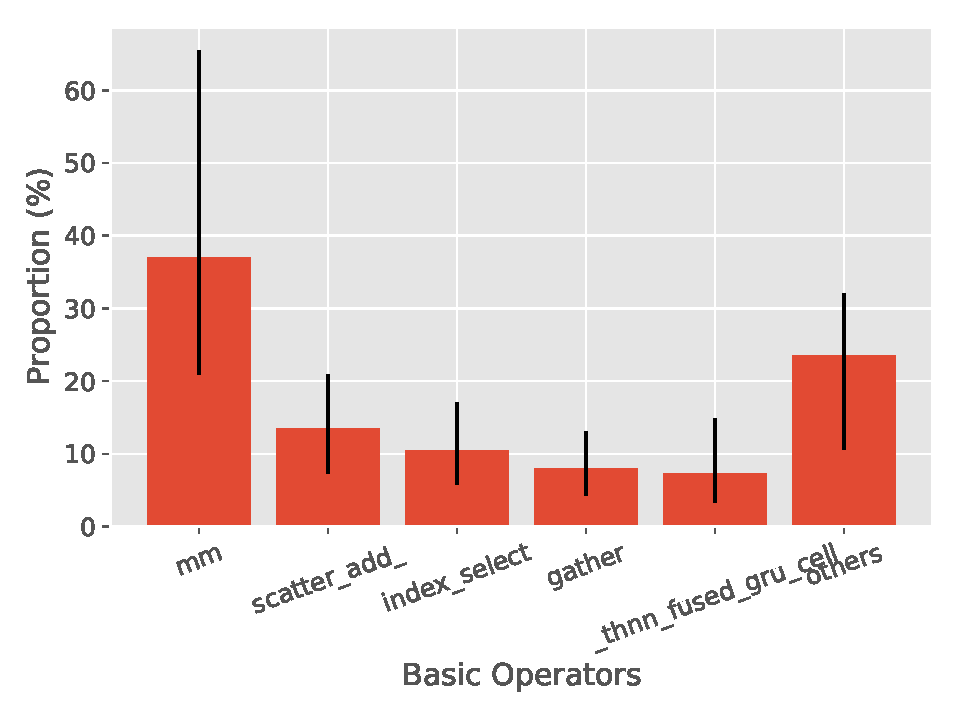
\includegraphics[width=0.35\columnwidth]{../figs/experiments/exp_inference_full_top_basic_ops_ggnn.pdf}}\\
        \subfloat[GAT, Training]{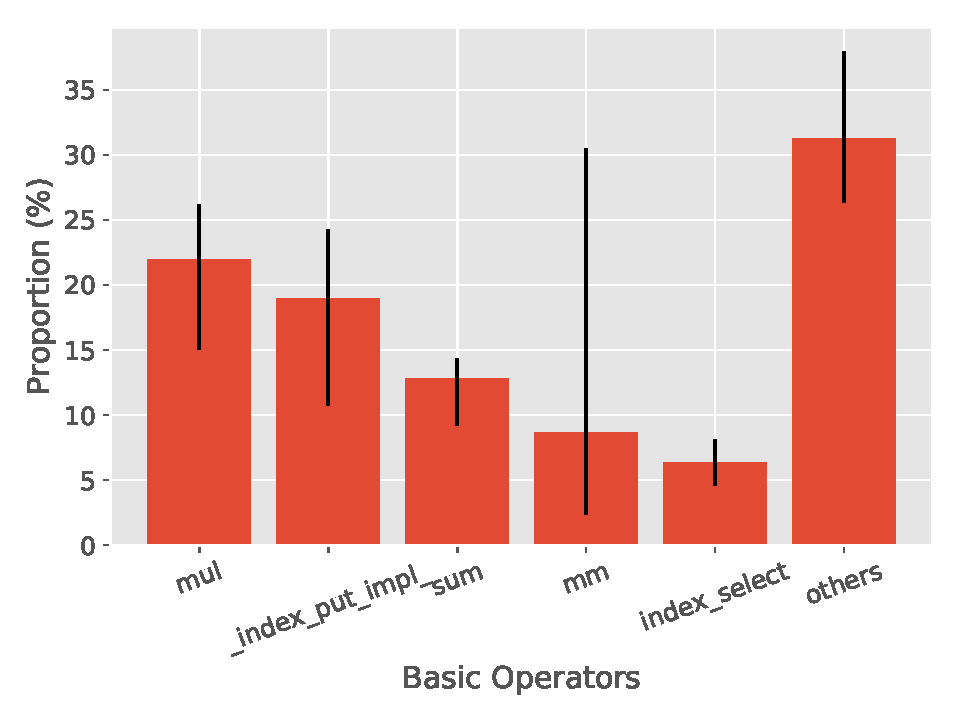
\includegraphics[width=0.35\columnwidth]{../figs/experiments/exp_top_basic_ops_gat.pdf}}
         \subfloat[GAT, Inference]{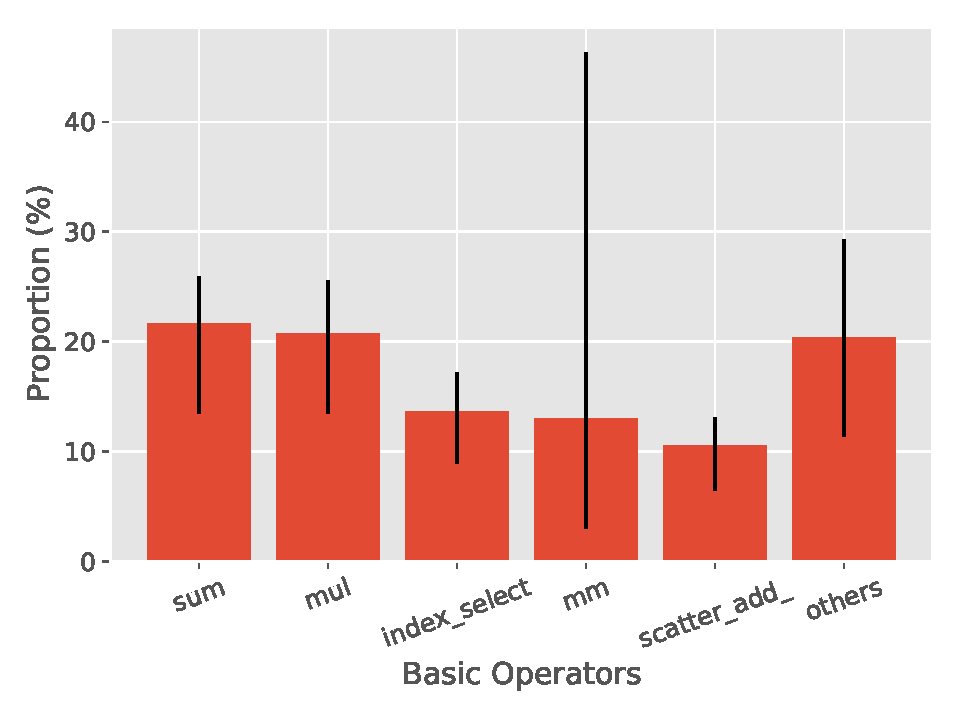
\includegraphics[width=0.35\columnwidth]{../figs/experiments/exp_inference_full_top_basic_ops_gat.pdf}}\\
        \subfloat[GaAN, Training]{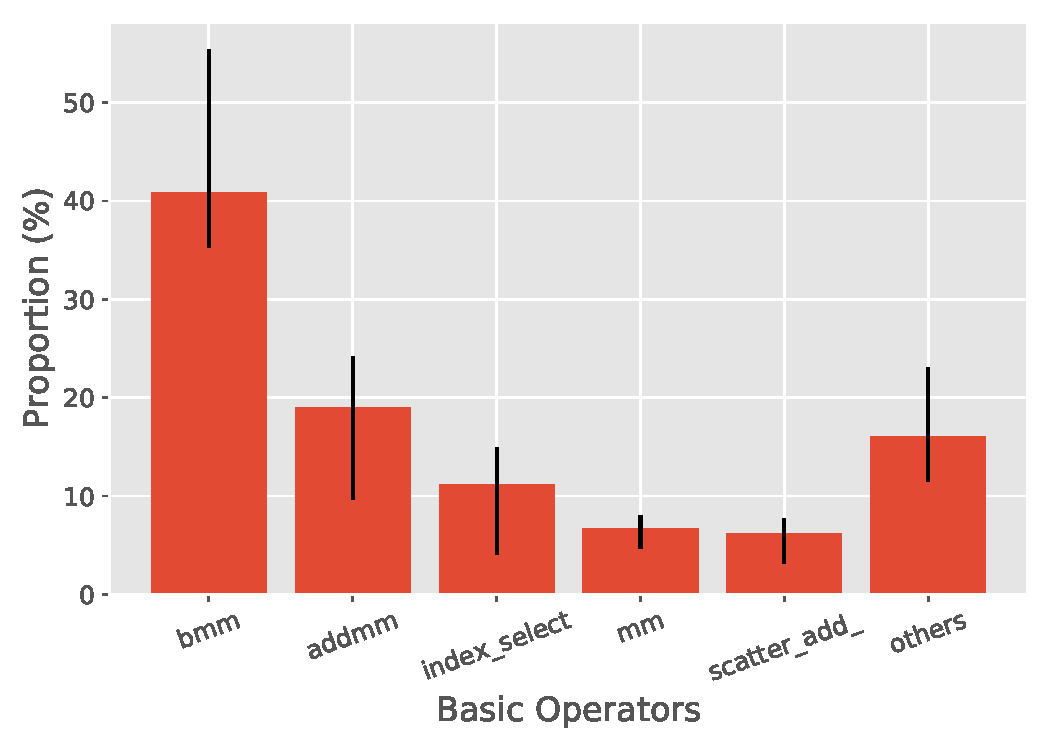
\includegraphics[width=0.35\columnwidth]{../figs/experiments/exp_top_basic_ops_gaan.pdf}}
         \subfloat[GaAN, Inference]{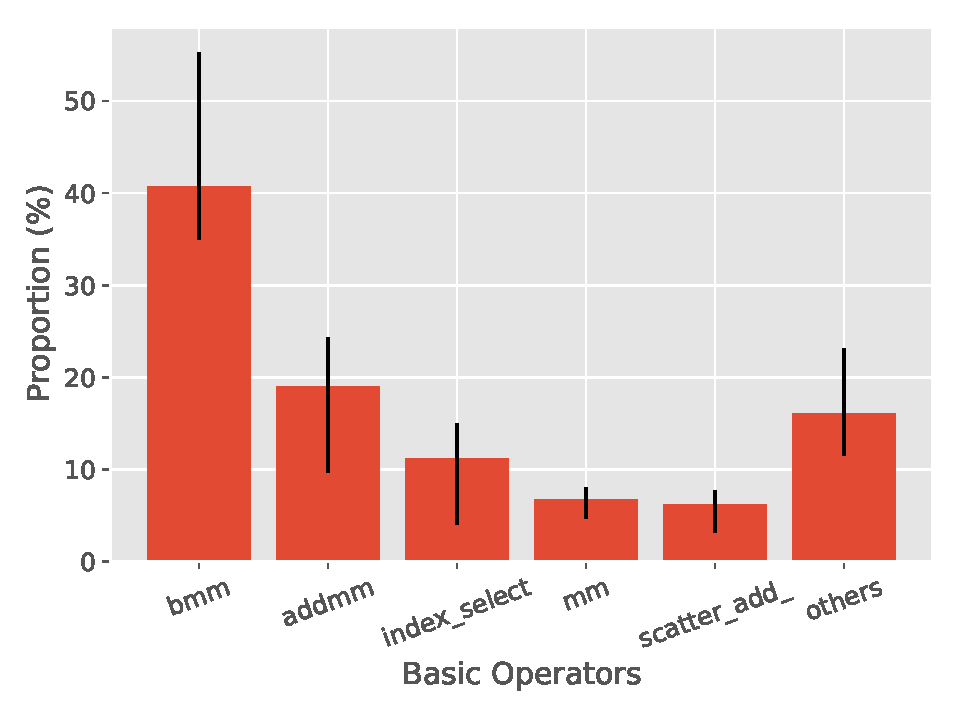
\includegraphics[width=0.35\columnwidth]{../figs/experiments/exp_inference_full_top_basic_ops_gaan.pdf}}\\
         
         \caption{Top 5 time-consuming basic operators of typical GNNs. The time proportion of each basic operator was averaged over all datasets with the error bar indicating the maximum and the minimum.}
         \label{fig:compare_top_time_consuming_basic_operators}
         
    \end{figure}
    
    \paragraph{Section 4.3 ``Memory Usage Analysis''}
         
     In Section 4.3 ``Memory Usage Analysis'', we have additionally conducted the memory usage analysis for GNN inference and added related discussion.
     %
     Figure~\ref{fig:compare_memory_expasion_ratio} in the response (Figure X in the revised manuscript) compares the memory expansion ratios of typical GNNs during training and inference.
     %
     Since no intermediate results had to be cached during inference, the memory expansion ratios of inference were much less than training for GGNN, GAT, and GaAN.
     %
     The MERs of inference were 45\% to 83\% (GGNN), 52\% to 61\% (GAT), and 37\% to 69\% (GaAN) of training.
     %
     However, the values of MERs were still high, disallowing inferencing with big graphs.
     
     \begin{figure}[H]
        \subfloat[Training]{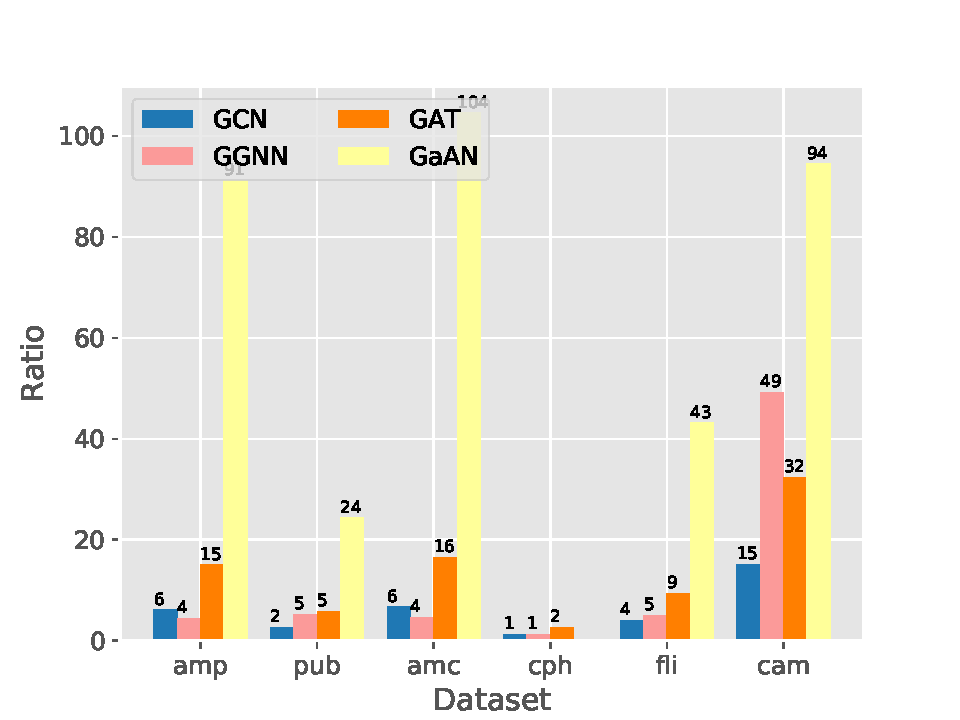
\includegraphics[width=0.5\columnwidth]{../figs/experiments/exp_memory_expansion_ratio.pdf}}
        \subfloat[Inference]{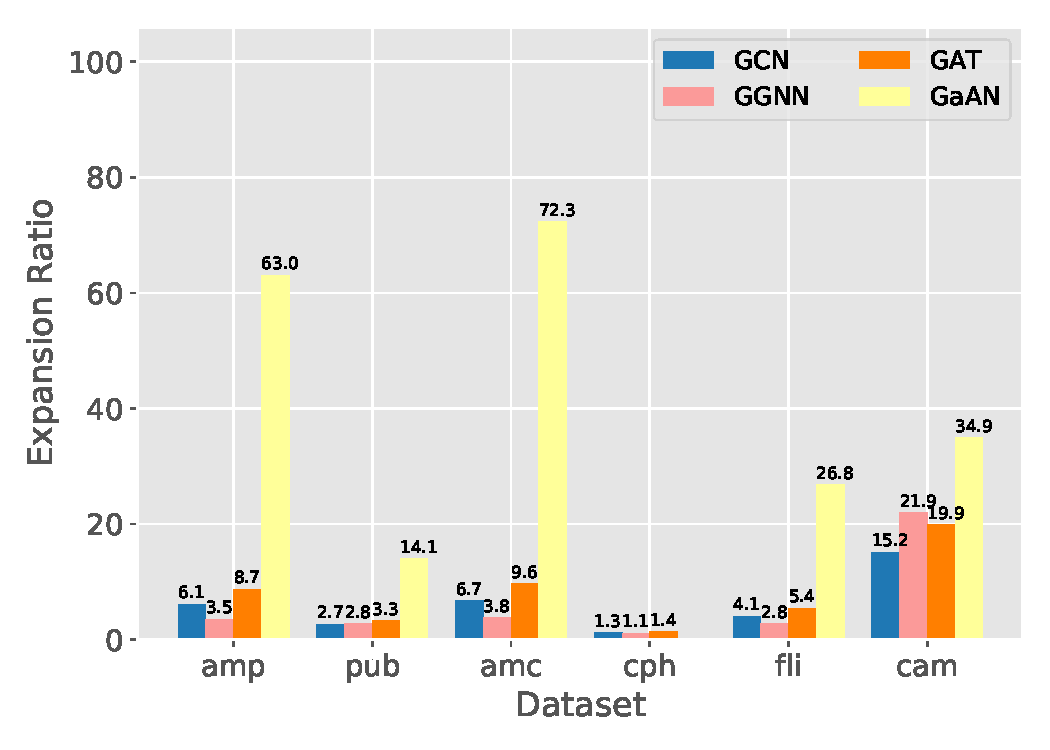
\includegraphics[width=0.5\columnwidth]{../figs/experiments/exp_inference_full_memory_expansion_ratio.pdf}}
        \caption{Memory expansion ratios of typical GNNs.}
        \label{fig:compare_memory_expasion_ratio}
     \end{figure}
     
     %%% TODO %%%
     
     \paragraph{Section 4.4 ``Effects of Sampling Techniques on Performance''}

     In Section 4.4 ``Effects of Sampling Techniques on Performance'', we have additionally evaluated the performance bottlenecks in sample-based GNN inference.
     %
     We find that ...
     %%% TODO %%%

\end{reply}

% Begin a new reviewer section
\reviewersection

\begin{point}
    In the paper, authors accomplished a unique study and analysis on GNN models training complexity.  The articles first review and development history of GNNs and creatively model all architectures as input layers, intermediate layers of graph neurons and prediction layers. And they quantitatively summarize the time and space complexity of 4 representative GNNs, including graph convolution, gated recurrent graph net, graph attention net and GraphSage. Most importantly, the article first break down complexity into operator level and offered analysis of good granularity, giving reader more guidance in future study. At last, the solid experiments included the study of effects of hyper-parameters and a comparison of two major sampling techniques: neighbor sampling and cluster sampling.
\end{point}

\begin{reply}
    Thank you for your positive comments on our manuscript.
    %
    We have carefully revised the manuscript according to your comments.
    %
    We have revised our manuscript according to your kindly suggestions.
    %
    Please see the detailed responses below.
    %
    We have highlighted our modification point by point in the annotated version of the manuscript by red squares.
\end{reply}

\begin{point}
    In general, the paper was well written and organized with good structure and clear narratives. Just some minor language errors like line Page 8, Line 208, "In active graph neurons" =\textgreater "Inactive graph neurons".
\end{point}

% R2Q1
\begin{reply}
    Thank you for pointing them out.
    %
    We feel really sorry for our carelessness.
    %
    We have proofread our revised manuscript carefully to eliminate such language errors as much as we can.
\end{reply}

% R2Q2
\begin{point}
    I was impressed by the way that authors categorize layers and operators in GNNs, very clear and instructive.
    
    It is also pretty neat to divide layer time complexity into two buckets: vertex calculation and edge calculation. The data model pretty well summarizes mainstream GNN layer architectures. And this analysis is very insightful for layer profiling.
    
    And the experimental evaluation were done over 6 large graph-structured datasets.
\end{point}

\begin{reply}
    Thank you very much for your appreciation.	
\end{reply}

% R2Q3
\begin{point}
    While, one major drawback is that I did not clearly see the analysis complexity v.s. accuracy. For example, in Figure 19 and 20, I did not see network accuracy from those 4 GNNs. There is always tradeoff between model complexity and model performance, and in some scenarios where high complexity is allowed, a sophisticated model of more powerful representation capability is still needed.
\end{point}

\begin{reply}
    Thanks very much for your valuable suggestions.
    %
    The model complexity directly affected both the accuracy and the training time.
    %
    In order to analyze the relationship between model complexity and accuracy, we conducted two kinds of extra experiments in the revised manuscript: (1) how the hyper-parameters of the GNNs (like the dimension of hidden vectors and the number of heads) affected the accuracy of GNNs (in Section 4.1); (2) how the batch size in the sampling methods affected the accuracy of GNNs (in Section 4.4).

    In this reply, we focus on the first kind of experiments added in Section 4.1.
    %
    We will introduce our results of the second kind of experiments in the nextR reply.

    In the revised manuscript, we added an extra paragraph ``Effects on Accuracy'' at the end of Section 4.1 ``Effects of Hyper-parameters on Performance'' to analyze how the hyper-parameters affect the accuracy.
    %
    We had two main findings: (1) the accuracy of GNNs was much more sensitive to the dimension of hidden vectors $dim(\MyVec{h}^1_x)$ (for GCN/GGNN/GaAN) and the dimension of each head $d_{head}$ (for GAT) than the other hyper-parameters; (2) the relative accuracy between the four typical GNNs varied greatly with different datasets.
    %
    We quote the related paragraphs from the revised manuscript below:

    \begin{myquote}{Test}
            %%% TO ADD QUOTE %%%
    \end{myquote}
\end{reply}

\begin{point}
    Sampling method is definitely going to reduce model complexity, since all models complexity depend on graph node number N, while performance is going to be compromised as well. I would like to see authors resolve the concern of significant accuracy drop after applying aggressive sampling of subgraphs.
\end{point}

\begin{reply}
    
\end{reply}

\begin{point}
    Hope authors supplement the effect of sampling and GNNs on accuracy while comparing different complexity of model and sampling methods.
\end{point}

\begin{reply}

\end{reply}

\end{document}